   The CLAS12 detector is a large angle spectrometer that generally covers angles from 5 to 130 degrees, spanned by two main detector subsystems - the Forward Detector and the Central Detector.

    Overview of Jefferson Lab
    Why is CLAS12 particularly suited for this measurement?

\section{Accelerator and Beamline}
    The Thomas Jefferson National Accelerator Facility, also called Jefferson Lab (JLab), is one of the 17 National Laboratories in the United States \parencite{DepartmentofEnergy2023DepartmentLaboratories}, and functions mainly to deliver high energy, continuous wave (CW) electron beams to fixed-target nuclear and particle physics experiments. The facility was established in 1984 - initially named the Continuous Electron Beam Accelerator Facility (CEBAF) - and first delivered a 4 GeV electron beam on July 1 1994 to one of its three original detector halls. In 2006 efforts began to upgrade the facility to produce an electron beam up to 12 GeV in energy, which was first successfully delivered in 2015, as well as to construct a fourth detector hall for additional physics experiments\parencite{JeffersonLab2023AboutLab}. JLab is also home to a free-electron laser, capable of 10+ kW CW operation \parencite{Benson2007HighAccelerator}. 

\begin{figure}[ht]
    \centering
    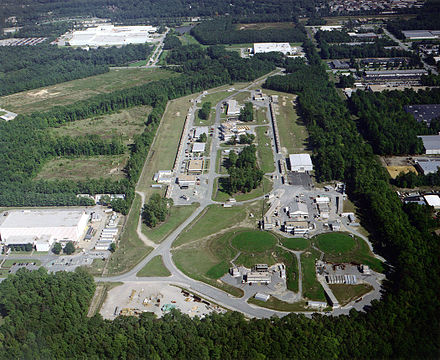
\includegraphics[width=0.8\textwidth]{Chapters/Ch2-Experiment/accel_and_beamline/pics/CEBAF/jlab_wiki.png}
    \caption{An aerial view of the Thomas Jefferson National Accelerator Facility \parencite{Wang2010CEBAFOverview}. Note that this picture was taken before the addition of the fourth detector hall (Hall D).}
    \label{fig:jlab_wiki}
\end{figure}

\subsection{Accelerator Facility}
    
    \figref{fig:jlab_accelerator_layout} shows the overarching scheme of the entire accelerator facility relevant for this experiment. Electrons are produced via the photoelectric effect from a 499 MHz pulsed laser impinges on a Gallium Arsenide photocathode (\figref{fig:gun}). The CEBAF guns operate at 100 kV and accelerate the electrons through a beam chopper (\figref{fig:chopper}) to create the desired beam structure (\figref{fig:structure}) and into the main accelerator circuit, where 1497 MHz superconducting resonator (SRF) cavities provide further acceleration (\figref{fig:klystron}). CEBAF's two $\sim$ 1.1 GV linacs accelerate electrons by consist of 50 cryomodules total, with each cryomodule housing 8 7-cell SRF cavities and the liquid helium necessary to cool them, made possible by JLab's 2K liquid helium refrigerator, the largest in the world as of 2023. The electrons are steered around the curved parts of the track by dipole magnets (\figref{fig:magnets}), making five complete circulations before delivery to the three western experimental halls.
    
    
    \begin{figure}[ht]
        \centering
        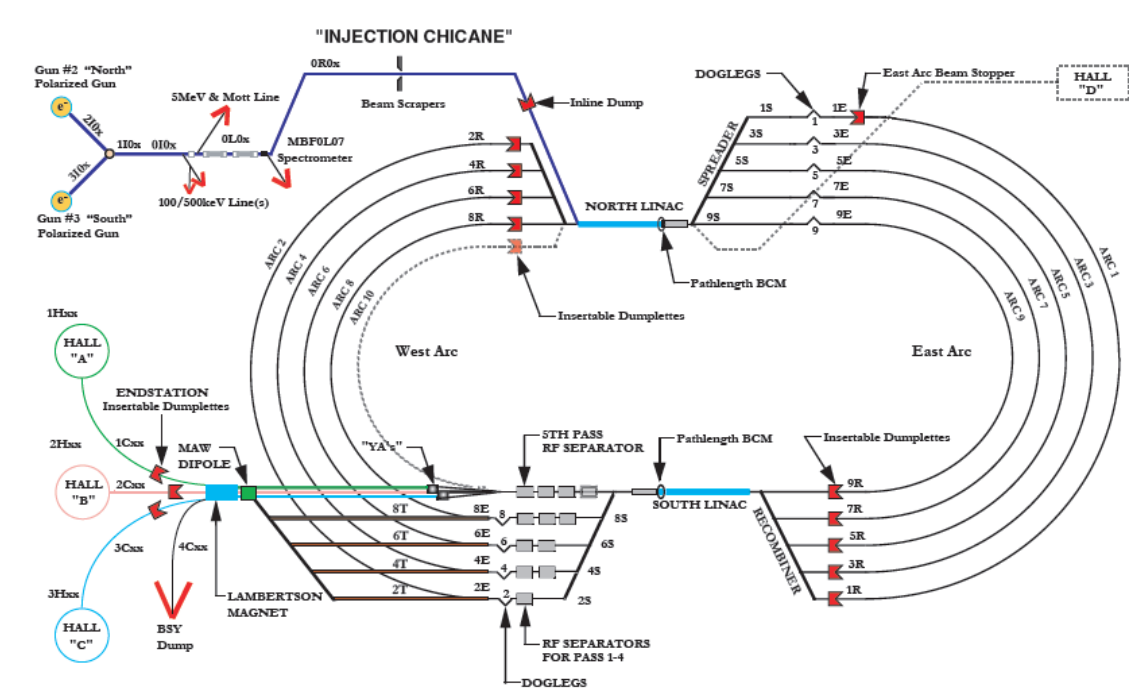
\includegraphics[width=0.8\textwidth]{Chapters/Ch2-Experiment/accel_and_beamline/pics/CEBAF/jlab-accelerator-layout.png}
        \caption{Schematic layout of the CEBAF accelerator at JLab. The racetrack configuration has two linear accelerator portions $\sim$ 1/4 mile long, and is $\sim$ 7/8 mile around \parencite{Wang2010CEBAFOverview}.}
        \label{fig:jlab_accelerator_layout}
    \end{figure}
    
    
    \begin{figure}[htb]
        \begin{minipage}[c]{\linewidth}
            \centering
            \subfloat[]{\label{fig:gun}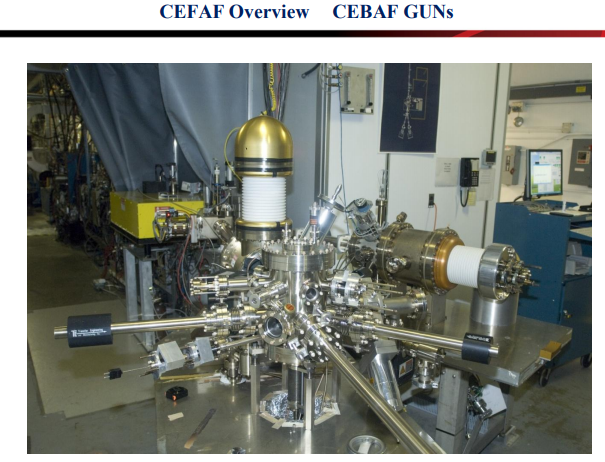
\includegraphics[width=0.3\textwidth]{Chapters/Ch2-Experiment/accel_and_beamline/pics/CEBAF/1_CEBAF-guns.png}}
            \subfloat[]{\label{fig:chopper}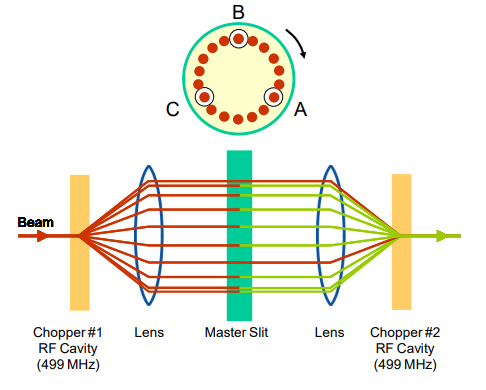
\includegraphics[width=0.3\textwidth]{Chapters/Ch2-Experiment/accel_and_beamline/pics/CEBAF/jlab-chopper.png}}
            \subfloat[]{\label{fig:structure}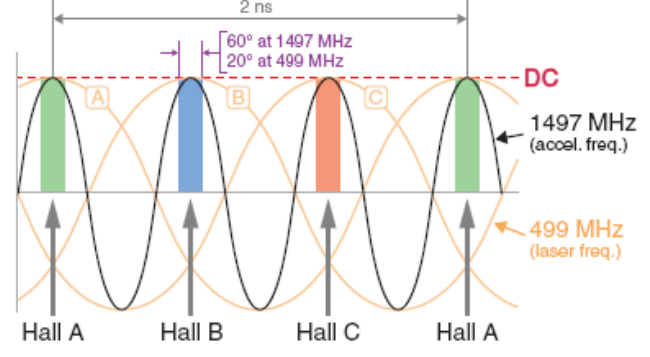
\includegraphics[width=0.3\textwidth]{Chapters/Ch2-Experiment/accel_and_beamline/pics/CEBAF/Jlab-beam-structure.png}}
        \end{minipage}
        \begin{minipage}[c]{\linewidth}
            \centering
            \subfloat[]{\label{fig:klystron}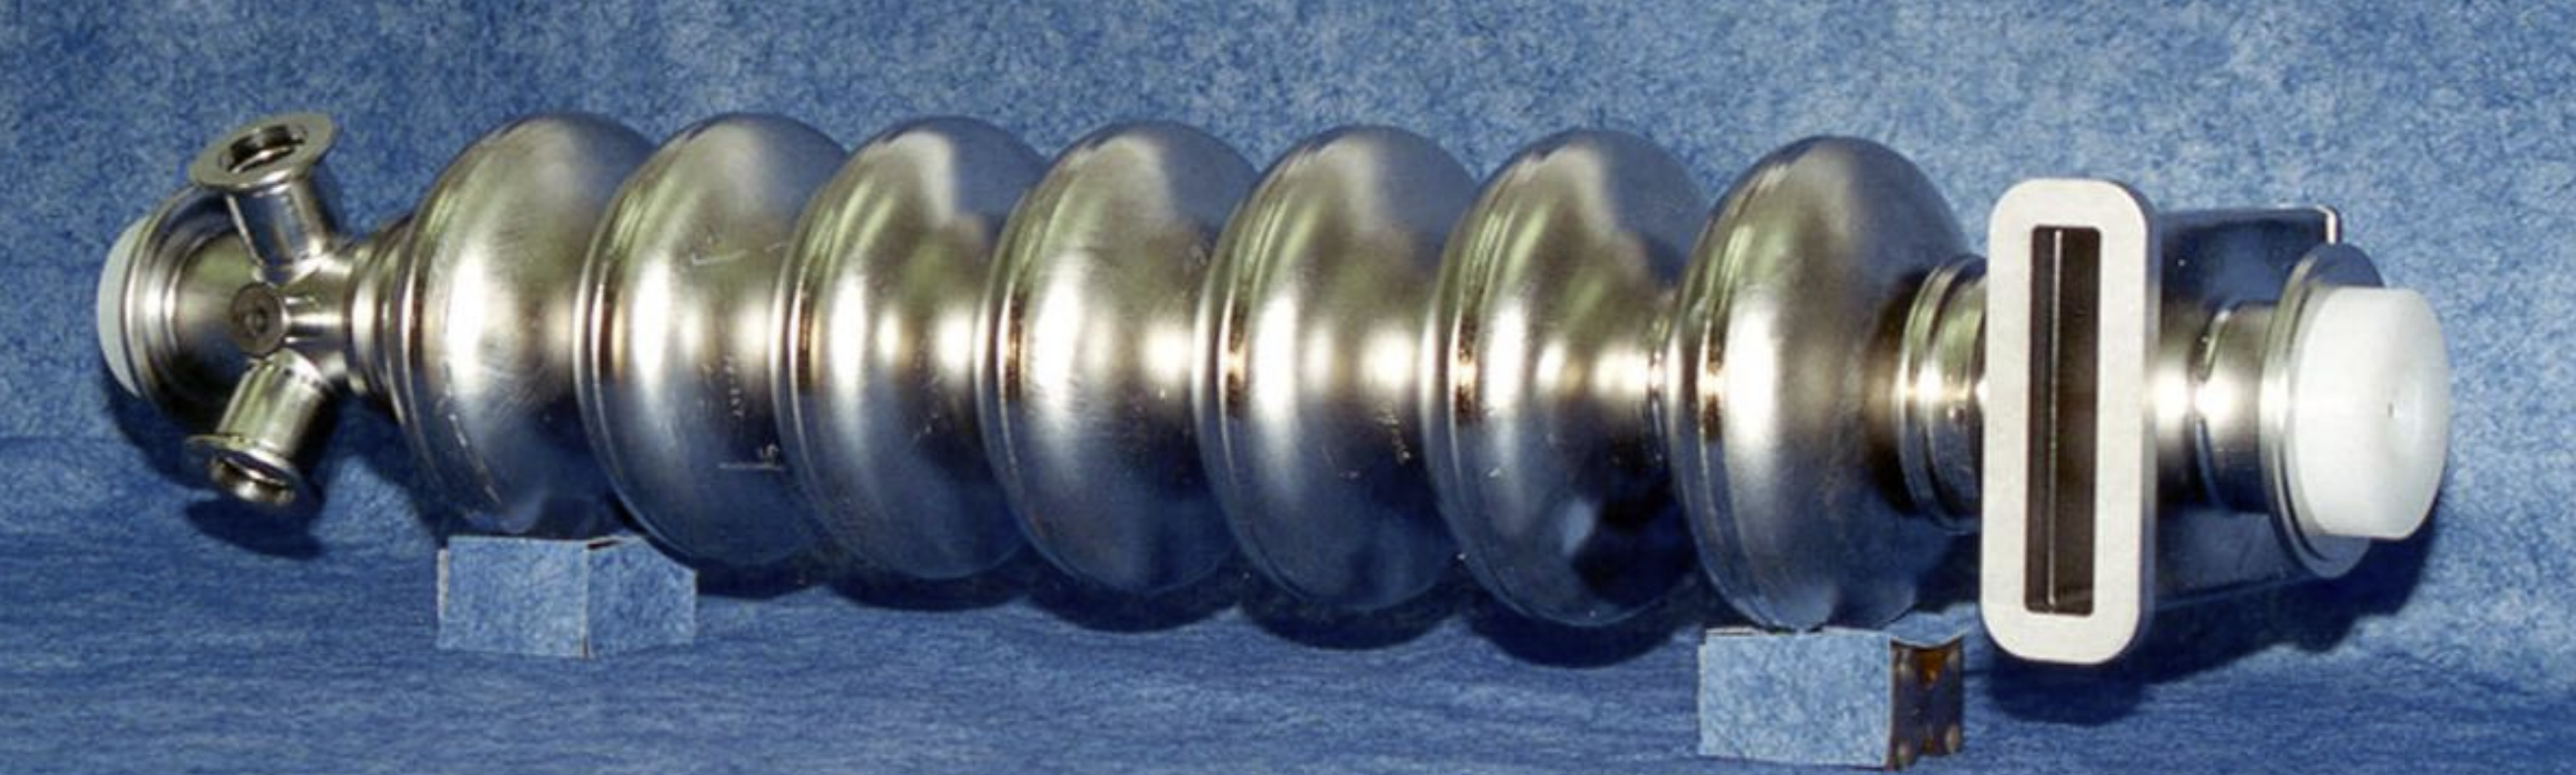
\includegraphics[width=0.4\textwidth]{Chapters/Ch2-Experiment/accel_and_beamline/pics/CEBAF/klystron.png}}
            \subfloat[]{\label{fig:magnets}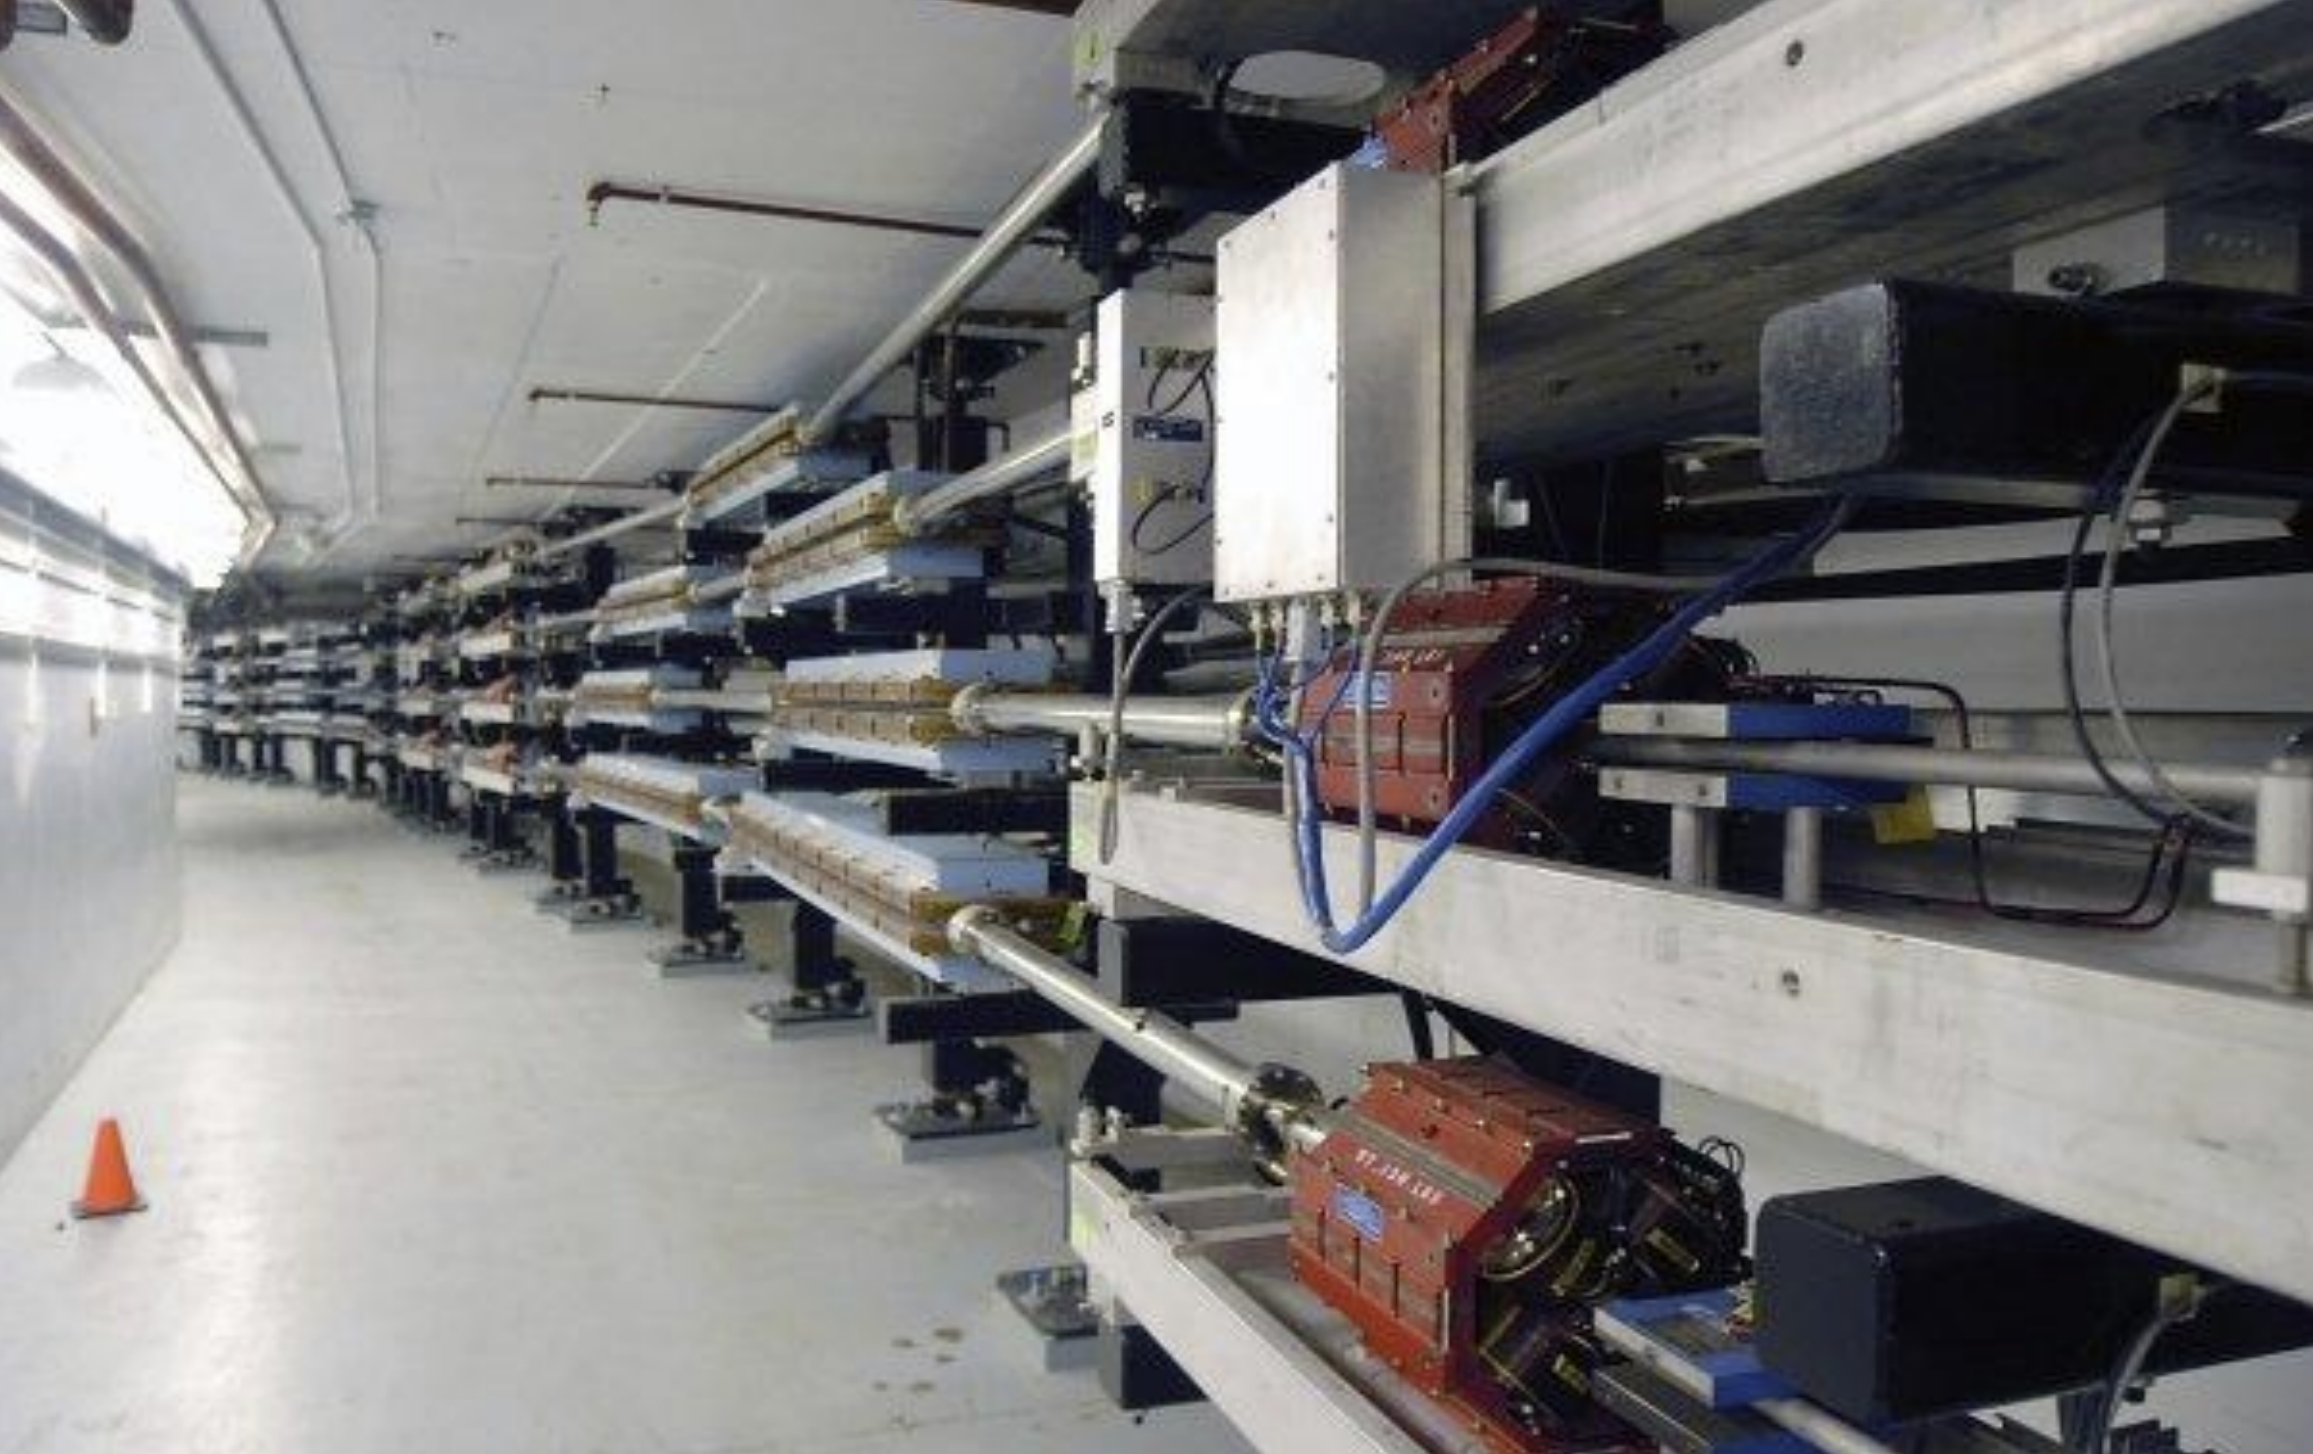
\includegraphics[width=0.4\textwidth]{Chapters/Ch2-Experiment/accel_and_beamline/pics/CEBAF/magnets2.png}}
        \end{minipage}
        \caption{(a) CEBAF guns, (b) Beam chopper, (c) Beam structure, (d) Superconducting resonator, (e) Dipole magnets.}
        \label{fig:JLab}
    \end{figure}
    

\subsection{Hall B Beamline}

    Moller polarimeters
    raster and target
    faraday cup / beamdump

    
    Finally, excess beam is safely managed using beam dumps. 
    
    \begin{figure}[ht]
        \centering
        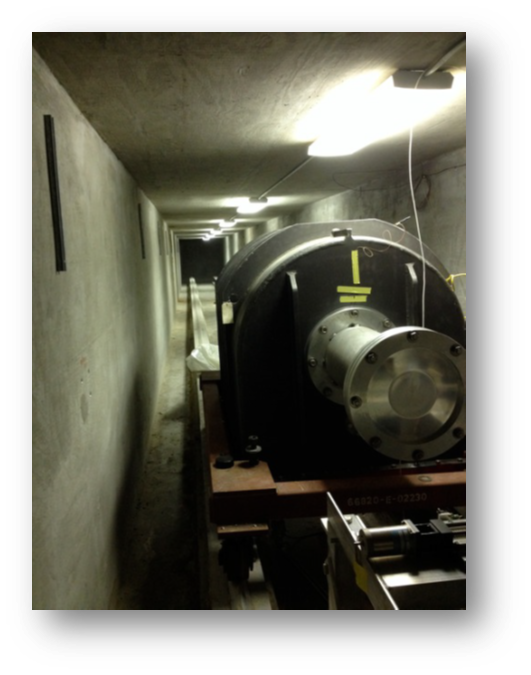
\includegraphics[width=0.8\textwidth]{Chapters/Ch2-Experiment/accel_and_beamline/pics/hallB/beamdump1.png}
        \caption{The first stage of the beam dump system at JLab.}
        \label{fig:beam_dump1}
    \end{figure}
    
    \begin{figure}[ht]
        \centering
        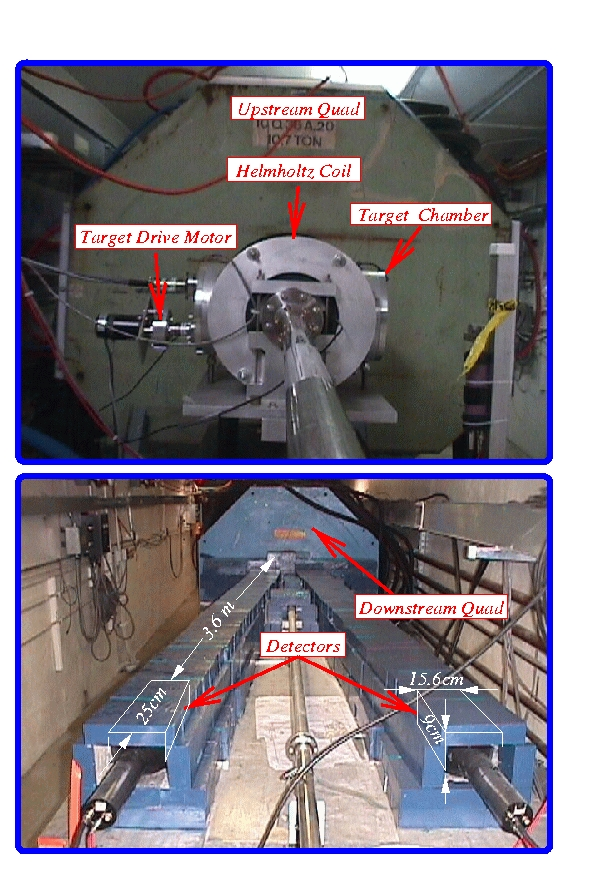
\includegraphics[width=0.8\textwidth]{Chapters/Ch2-Experiment/accel_and_beamline/pics/hallB/hall-b-poll-2.jpg}
        \caption{Moller polarimeters}
        \label{fig:beam_dump1}
    \end{figure}

    
    \begin{figure}[ht]
        \centering
        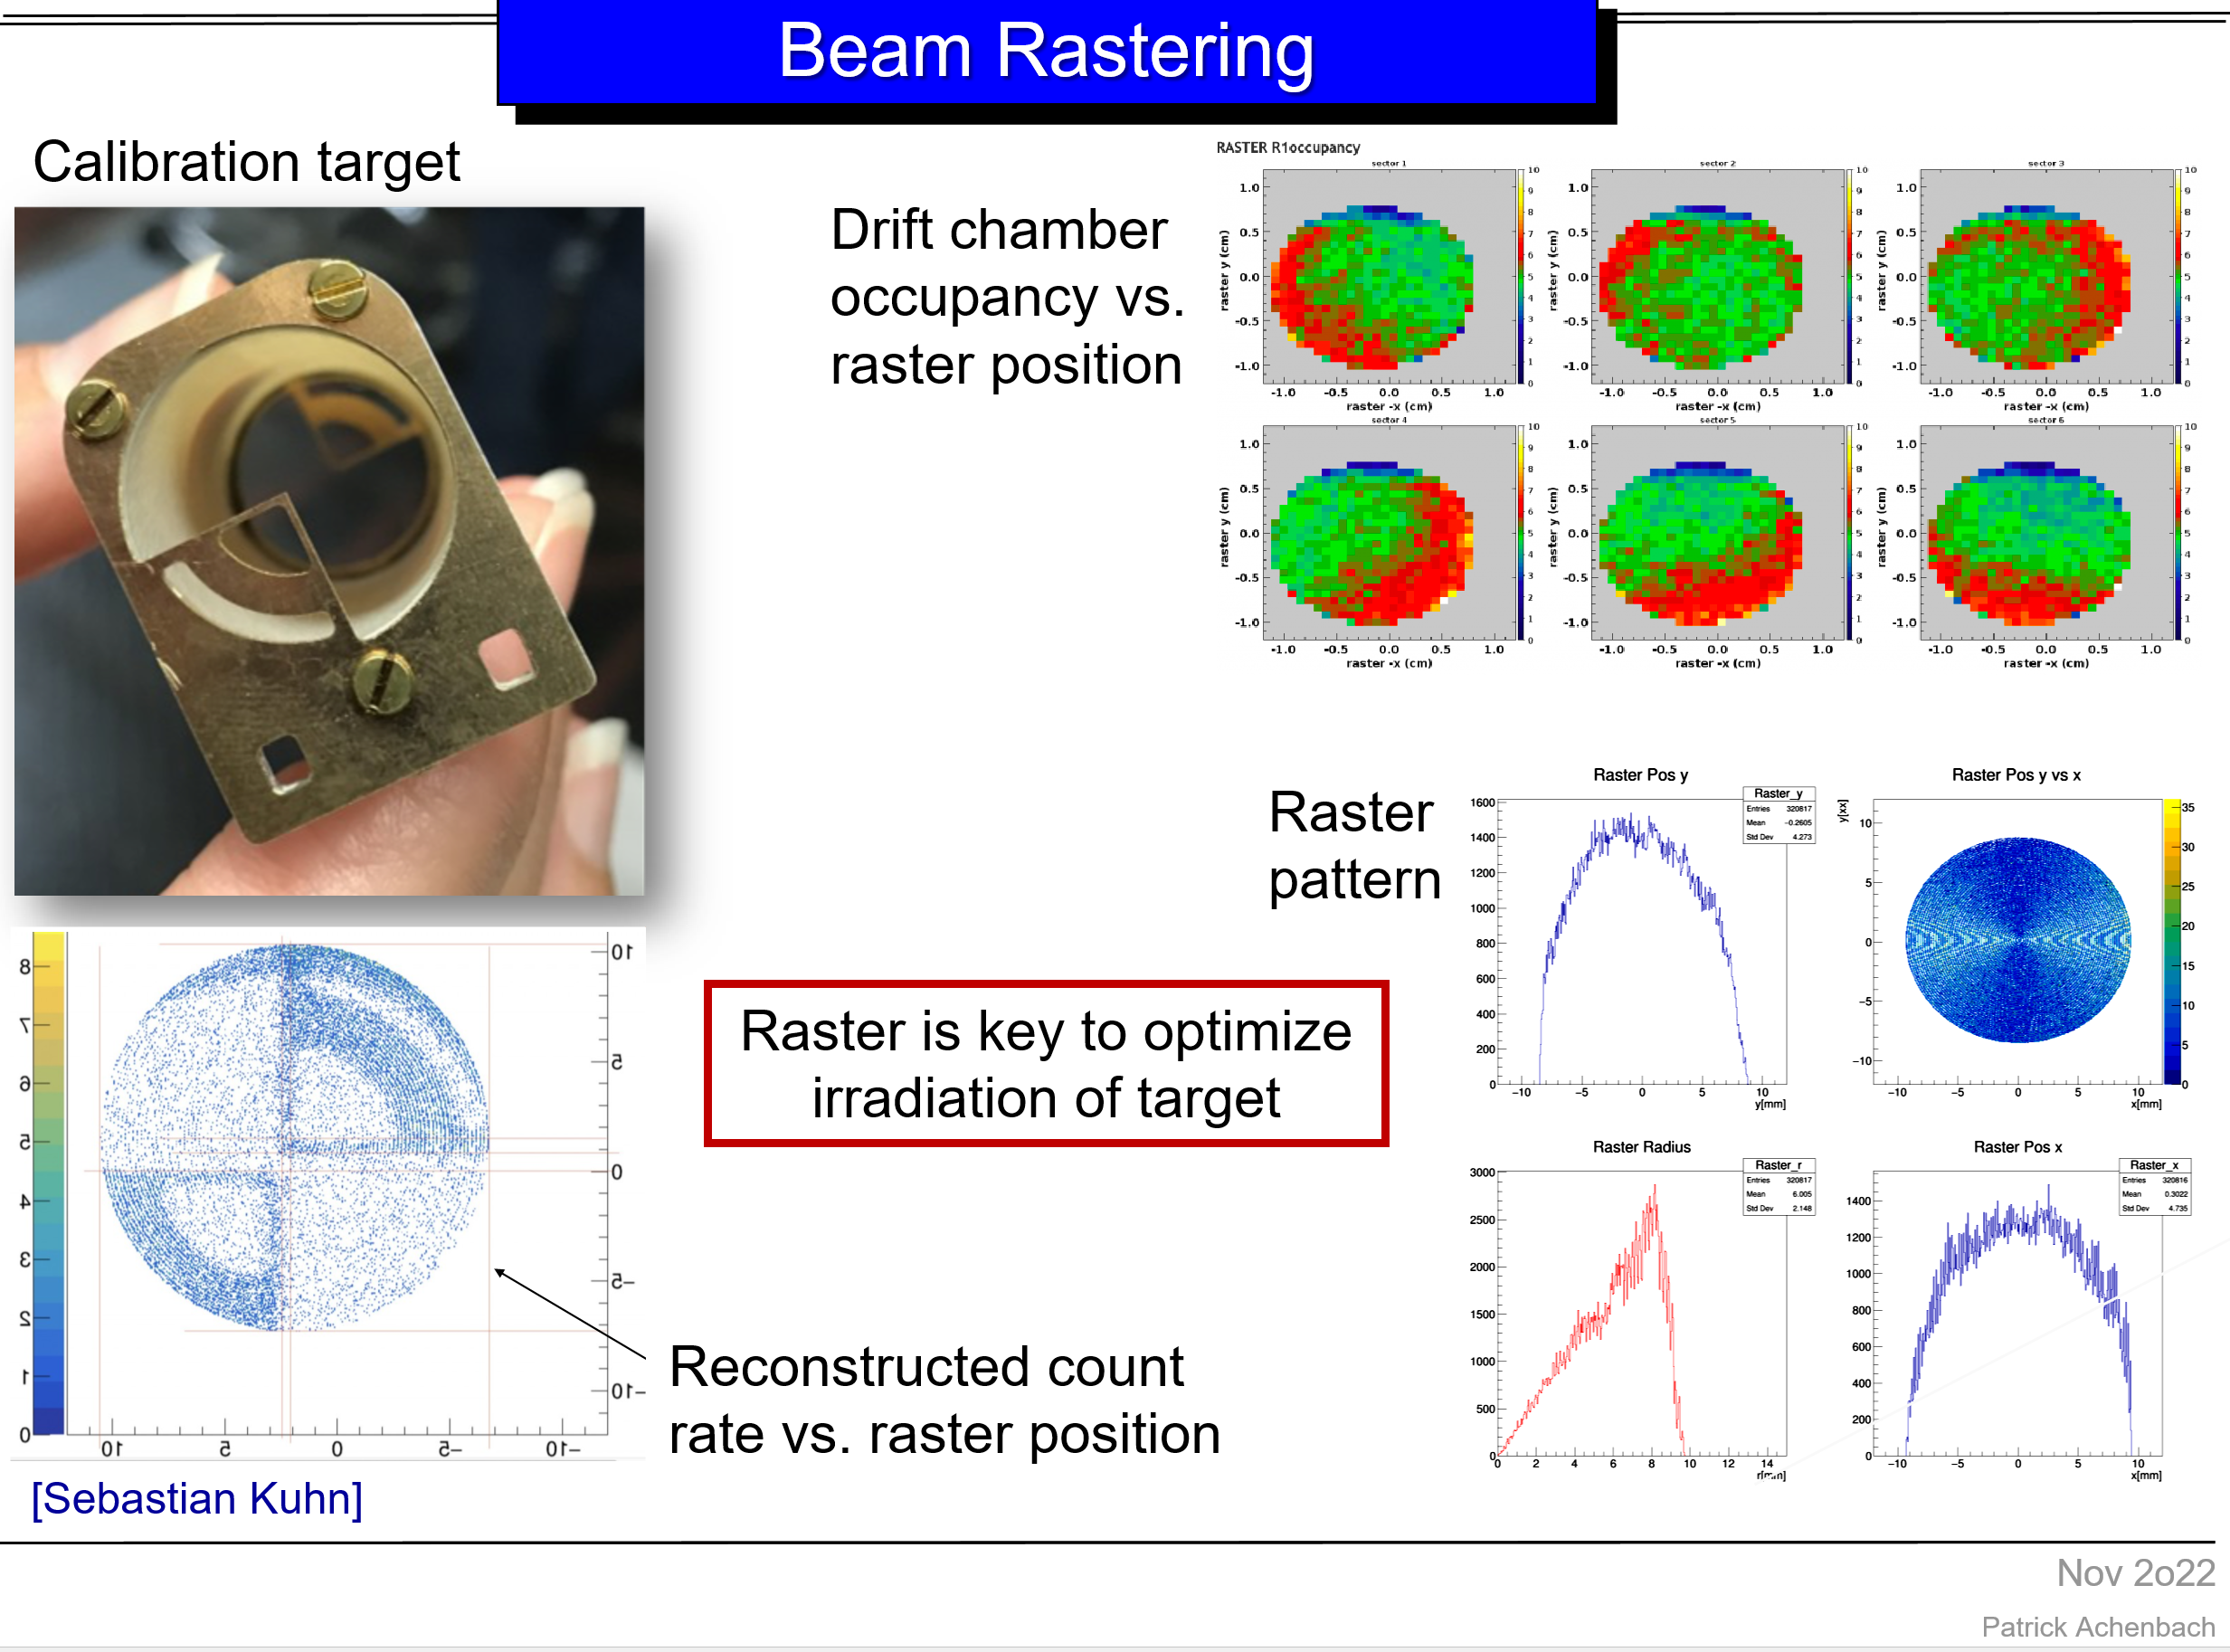
\includegraphics[width=0.8\textwidth]{Chapters/Ch2-Experiment/accel_and_beamline/pics/hallB/beam_rastering.png}
        \caption{The second stage of the beam dump system at JLab.}
        \label{fig:rastering}
    \end{figure}
    
    
    
        in beam dump area, link to own fraday cup paper \cite{Johnston2019RealizationElectrons}
        
    
    For entry into CLAS12, the beamline specs are as follows:\\
                        Beam current: up to 50 nA\\
                        Beam energy spread: $10^-4$\\
                        Beam size: Less than 0.4 mm\\
                        Beam stability: Less than 0.1 mm\\
                        Beam halo: $10^-4$\\
                        Beam polarization: up to 85\%\\
                        
    
    
    
    
    
     As stated, for RGA, the fact that the beam is polarized is not useful, but it is true and is measured by Moller Polarimeters. 
            
                Polarimietry: 
                        Good for beam energies between 100 MeV and 50 GeV. Polarized beam electrons are scat-
                tered from other polarized electrons in a target, usually magnetized foils. Only a small
                fraction of all the target electrons are polarized, so this method has a small analyzing
                power. Analyzing power is exactly calculable in QED. At high beam energies, analyzing
                power and scattering probability both become independently of beam energy. Maximum
                analyzing power is about 80%, maximum is at 90 degrees scattering angle in C.o.M. Trans-
                versely polarized target can be used to measure transverse beam polarization, but analyzing
                power is only about 10%. 90 degrees C.o.M. translates to a small lab angle with each elec-
                tron at half beam energy, so magnets are used to bend these electrons out to detectors.
                These detectors can be, for example lead glass total absorption cherenkov counters.Since
                the two electrons are corellated, can use things like time coincidence to reduce background,
                although for low duty factor accelerators only one electron is required as statistics would
                otherwise be too low.A main background to this process is Mott scattering with the electron
                radiating off energy after scattering, appearing as a Moller electron
                
                The scattering target is either iron or vanadium permendur (iron-cobalt alloy). Only 2 of
                26 electrons in iron have their spins oriented, leading to a total analyzing power of only 6 percent
                and transverse analyzing power of only 1%. Uncertainties in how magnetized the targets
                actually are corresponds to an uncertainty in analyzing power. There are ’easy’ and ’hard’
                magnetization schemes - easy does a soft magnetization, while hard uses a several tesla mag-
                net to saturate the target. In principle, uncertainties on magnetization in the hard scheme
                can be removed by using the Kerr magneto-optic effect, but this has not ever been imple-
                mented. An important correction is due to the Levchuk effect, where due to momentum
                differences between electrons in different shells, electrons scattered off of polarized electrons
                are more likely to be detected than off of unpolarized electrons. Specifically, inner electrons
                are unpolarized and have a large average momenta, so when struck they can fall outside the
                113 TOC
                acceptance of the Moller detectors, while the outer electrons, which are polarized, have a
                small average momentum, and behave as expected. This is up to a 15% effect on polarization
                measurements, and is currently a work in progress.
    
    
                
    
                 Rasterization of some kind
                    \\
                    \indent The hydrogen target in RGA is cooled to 20 K using a He4 evaporation fridge. Can by polarized by dynamic nuclear polarization, driven by a 140 GHz microwave source, can reach 90\% polarization for protons, 40\% for deuterons (both longitudinally polarized). The polarization can be measured by a Q-meter based NMR. 2.5 cm diameter target, extended 5 cm long. \\
                    \indent RGA does not use a polarized target. The beam is polarized, but the target is not, so polarization is not helpful for extracting the 5-fold differential cross section (but it would be if the target was also polarized, and is useful for BSA measurements).
                
       
                Luminosity in CLAS12 is measured from the Faraday Cup and using reference reactions such as elastic scattering. We don't use the Faraday Cup event by event, but we do use it run by run. For beam current measurements, beam position monitors upstream are used - but this is for monitoring on-line, not for analysis.
                           Can manage 175 Watts - 17 nA at 10 GeV. Is used to calibrate beam current, needs a blocker in at higher currents

\cleardoublepage
                                         

\section{CLAS Detectors and Run Conditions}\label{sec:clas12exp}
    The CEBAF Large Acceptance Spectrometer, 12 GeV (CLAS12) detector occupies experimental Hall B at Jefferson Lab. It is an upgrade from its predecessor, the CLAS detector \parencite{Mecking2003TheCLAS}, which operated in the 2000s during the 6 GeV era of JLab and laid the groundwork for the present detector system, which was commissioned in 2018. It covers nearly 4$\pi$ around the target cell, with comprehensive packages of detectors for particle position and energy tracking. It operates with data rates of comparable size to other large-scale, international physics experiments, as shown in \tabref{table:experiments}. Data taking began in 2018 and has an experimental program approved into at least the early 2030s \parencite{Battaglieri2021PresentProgram}.

\iffalse
%Differences between clas and clas12 detectors
CLAS12 acceptances and resolutions are also superior to that of CLAS6. Main differences are:
- RGK has outbending torus vs inbending CLAS6 data
- the distance between the target and the PCal has increased, the FTCal extends to lower angles, and the gap between FTCal and PCal is much smaller than between IC and EC
- proton polar angle was limited to 60 deg in the e1dvcs dataset if my memory is correct
\fi


\begin{table}[h]
    \centering
    \begin{tabular}{l|lccc}
         \headercell{\textbf{Facility}} & \textbf{Experiment} &  \headercell{\textbf{Event Size} \\ \textbf{(kB)}}  &  \headercell{\textbf{L1 Trigger Rate} \\ \textbf{(kHz)}}  &  \headercell{\textbf{Bandwidth to Storage} \\ \textbf{(MB/s)}}      \\ \\ \hline
        JLab & GlueX & 15 & 200 & 300 \\
        JLab & \textcolor{purple}{\textbf{CLAS12}} & \textcolor{purple}{\textbf{20}} & \textcolor{purple}{\textbf{10}} & \textcolor{purple}{\textbf{100}} \\
        LHC & ALICE & 2,500 & 200 & 200 \\
        LHC & ATLAS & 1,500 & 75 & 300 \\
        LHC & CMS & 1,000 & 100 & 100 \\
        LHC & LHCb & 40 & 1,000 & 100 \\
        BNL & STAR & 1,000 & 0.6 & 450 \\
        BNL & PHENIX & 60 & 15 & 450 \\
    \end{tabular}
\caption[Data rates of various physics experiments]{Assorted physics experiments and their typical data rates. Note that exact figures vary by source and run conditions. Adapted from \parencite{DavidLawrence2012TheLab}.}
\label{table:experiments}
\end{table}

\subsection{CLAS12 Detector System}
    The CLAS12 detector \figref{fig:clas12photo} has two major subsystems: the Forward Detector and the Central Detector, as well as a forward tagger (nested inside the forward detector package) and backward angle neutron detector (BAND). 



\begin{figure}[H]
    \centering
    \subfloat[CLAS12 CAD layout.]{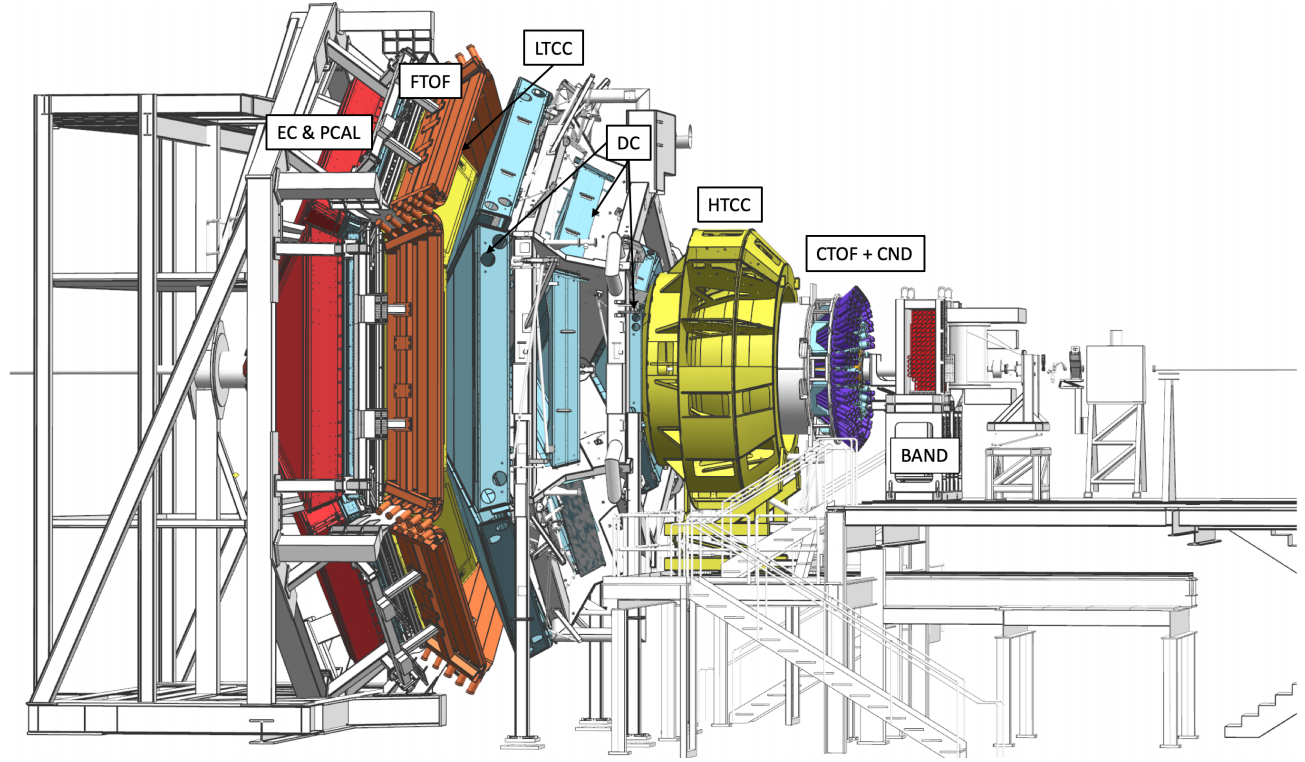
\includegraphics[width=0.45\textwidth]{Chapters/Ch2-Experiment/clas-12-exp/clas-detectors/other/pics/CLAS12.png}\label{fig:clas12}}
    \hfill
    \subfloat[CLAS12, fully installed.]{\includegraphics[width=0.45\textwidth]{Chapters/Ch2-Experiment/clas-12-exp/clas-detectors/other/pics/clas-real.png}\label{fig:clas12spec}}
    \caption[CLAS12 Layout]{CLAS12 layout schematic and photograph, from \parencite{Burkert2020TheLaboratory}.}\label{fig:clas12photo}
\end{figure}



\subsubsection*{Forward Detector}

    The Forward Detector (FD) is a 6-fold azimuthally symmetric segmented system containing several detector packages and a toroidal magnet. The sections follow a counterclockwise numbering convention where S1 corresponds to $[-30^{\circ}, 30^{\circ}]$, as in \figref{fig:fd_sections}. Working from the target downstream, the FD consists of a High Threshold Cherenkov Counter (HTCC) \parencite{Sharabian2020TheCounter}, Low Threshold Cherenkov Counter (LTCC) \parencite{Ungaro2020TheDetector}, the Ring Imaging Cherenkov detector (RICH) \parencite{Contalbrigo2020TheDetector}, Forward Time-of-Flight (FTOF) \parencite{Carman2020TheSystem}, Drift Chambers (DC) \parencite{Mestayer2020TheSystem} embedded in a 3.5 Tesla torodial magnetic field \parencite{Fair2020TheMagnets}, and Electromagnetic Calorimeter (ECal) complex \parencite{Asryan2020TheCalorimeter}.

    The ECal consists of three layers, two of which are from the previous CLAS experiment \parencite{Amarian2001TheCalorimeter}. Those two layers were only sufficient to contain showers with energies below 5 GeV, so a third layer (Pre-shower Calorimeter, PCal) was added to address this issue, as well as introduce the finer grained segmentation necessary to resolve the angle between the two photons of a neutral pion decay, which is of special importance for this process measurement. The FD system covers approximately $5^{\circ}$ to $35^{\circ}$ in polar angle, with one layer of the FTOF (FTOF-2) extending coverage to $45^{\circ}$. 
    
    %Likewise, the FTOF has three layers---FTOF 1a, FTOF 1b, and FTOF 2. The LTCC and the RICH were not used in this measurement.
               
    \begin{figure}[H]
        \centering
        \subfloat[FD sectioning.]{
            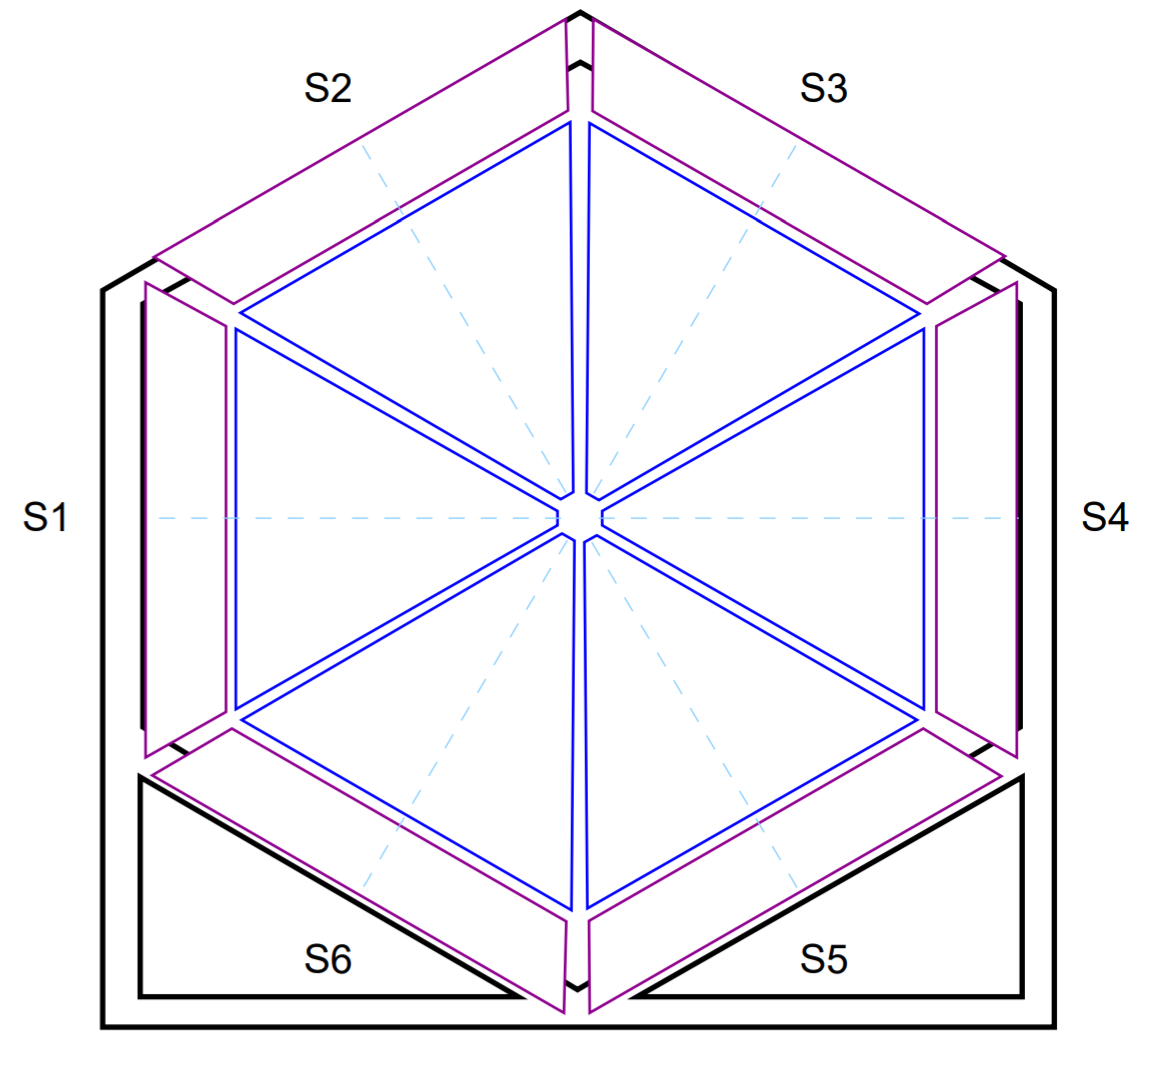
\includegraphics[width=0.3\textwidth]{Chapters/Ch2-Experiment/clas-12-exp/clas-detectors/fd/pics/ftof-front.png}\label{fig:fd_sections}
        }
        \hfill
        \subfloat[Model of HTCC.]{
            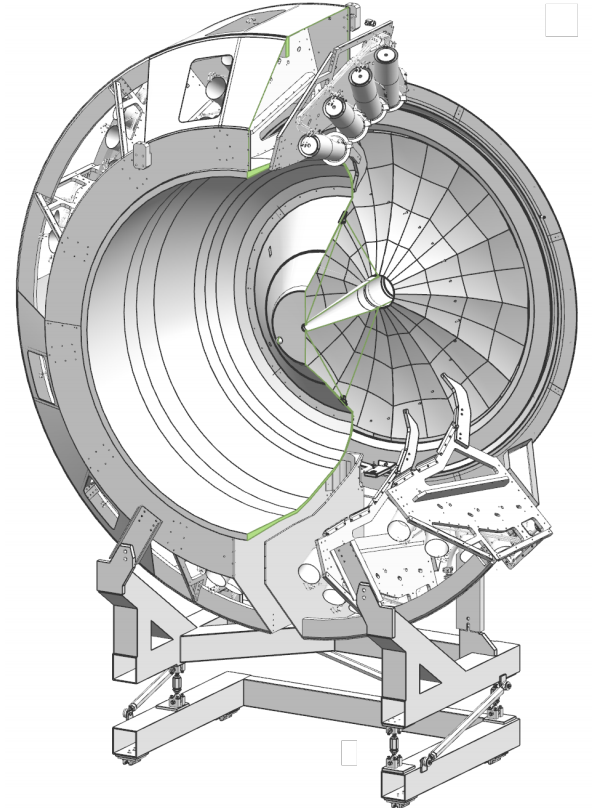
\includegraphics[width=0.3\textwidth]{Chapters/Ch2-Experiment/clas-12-exp/clas-detectors/fd/pics/htcc.png}\label{fig:htcc}
        }
        \hfill
         \subfloat[PCal and ECal assembly.]{
            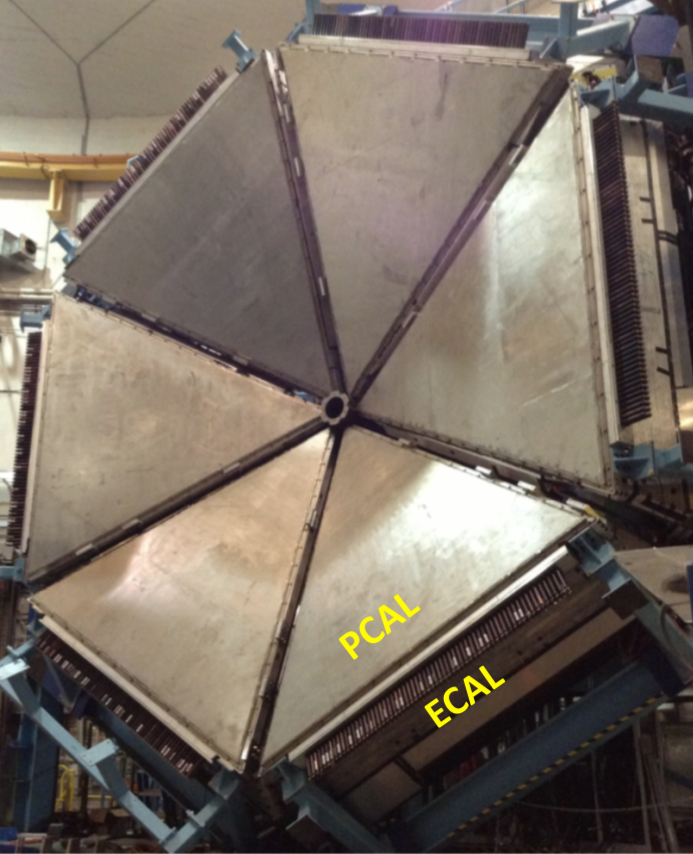
\includegraphics[width=0.3\textwidth]{Chapters/Ch2-Experiment/clas-12-exp/clas-detectors/fd/pics/clas12-pcal-ecal.png}\label{fig:pcalecal}
        }
        \caption[Forward Detector Packages]{The FD is broken into six sections (a), with the exception of the first component after the target, the HTCC (b). The PCal was added to the ECal from the CLAS experiment to achieve the necessary particle resolution. From \parencite{Burkert2020TheLaboratory}}
        \label{fig:select_FD_components}
    \end{figure}




\subsubsection*{Central Detector}

    The Central Detector (CD) also provides nearly 2$\pi$ azimuthal coverage, and spans from $\sim$ $35^{\circ}$  to $125^{\circ}$ in polar angle. The CD is an approximately 1 meter long cylinder inside a 5 Tesla solenoidal magnet \parencite{Fair2020TheMagnets} with four sub-detector packages. From the target working out, the packages are a Central Vertex Tracker \figref{fig:mvt}, made of a Barrel Micromegas Tracker (BMT) \parencite{Acker2020TheTracker} and Silicon Vertex Tracker (SVT) \parencite{Antonioli2020TheTracker}, a Central Time-of-Flight (CTOF) \parencite{Carman2020TheSystem} \ref{fig:ctof}, and a Central Neutron Detector (CND) \parencite{Chatagnon2020TheDetector}, which was installed but not used in this measurement. 
    
    %The main part is the SVT, while the BMT is used to improve the track reconstruction. 

    Low momentum transfer t \eqref{eq:t_momentum_trans} events correspond to large proton polar angles, meaning the majority of low-t events occur with a proton detected in the CD. These events are important as the GPD interpretation of deeply virtual processes is only valid in the regime where $\frac{-t}{Q^2}$ is small, and as such the CD is invaluable to acquiring data to gain insight on these distributions.        


        %CTOF
        %    Central for PID purposes. Divides into 48 1 meter long plastic scintillators with double sided PMT readout.PMTs are in the 0.1 T fringe field region and enclosed in magnetic shielding. 65 picosecond timing resolution. 35 to 125 degrees, 2 $\pi$ in polar angle. 3 cm x 3 cm scintillator planks. Pion/Kaon separation up to 0.64 GeV, Kaon/proton separation up to 1 GeV, pion proton separation up to 1.25 GeV.  	

 
        
        %Solenoid
	%	    5 Tesla super conducting magnet, uniform field ($\Delta$B/B = $10^-4$). Weakest at small angles, strongest at large angles. Opening polar angle of 40 degrees. Momentum range of interest 0.3 to 1.3 GeV. 18 Megajoules stored energy. 85 cm in diameter, 4.2 Kelvin operation. 


        \begin{figure}[H]
            \centering
            \subfloat[Model of CTOF.]{
                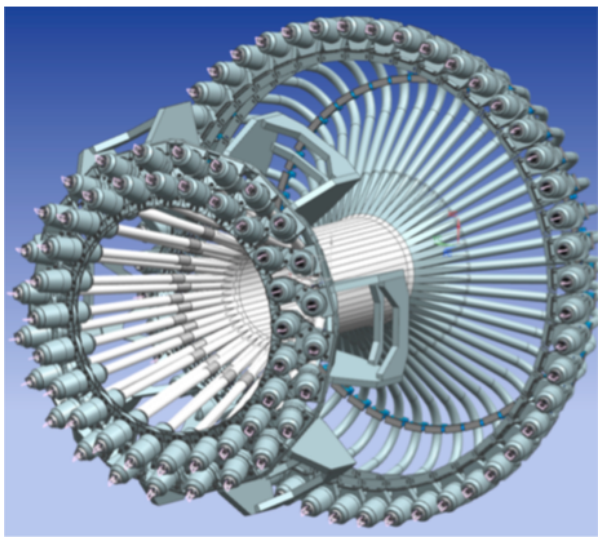
\includegraphics[width=0.3\textwidth]{Chapters/Ch2-Experiment/clas-12-exp/clas-detectors/cd/pics/CTOF.png}\label{fig:ctof}
            }
            \hfill
            \subfloat[Schematic of CVT.]{
                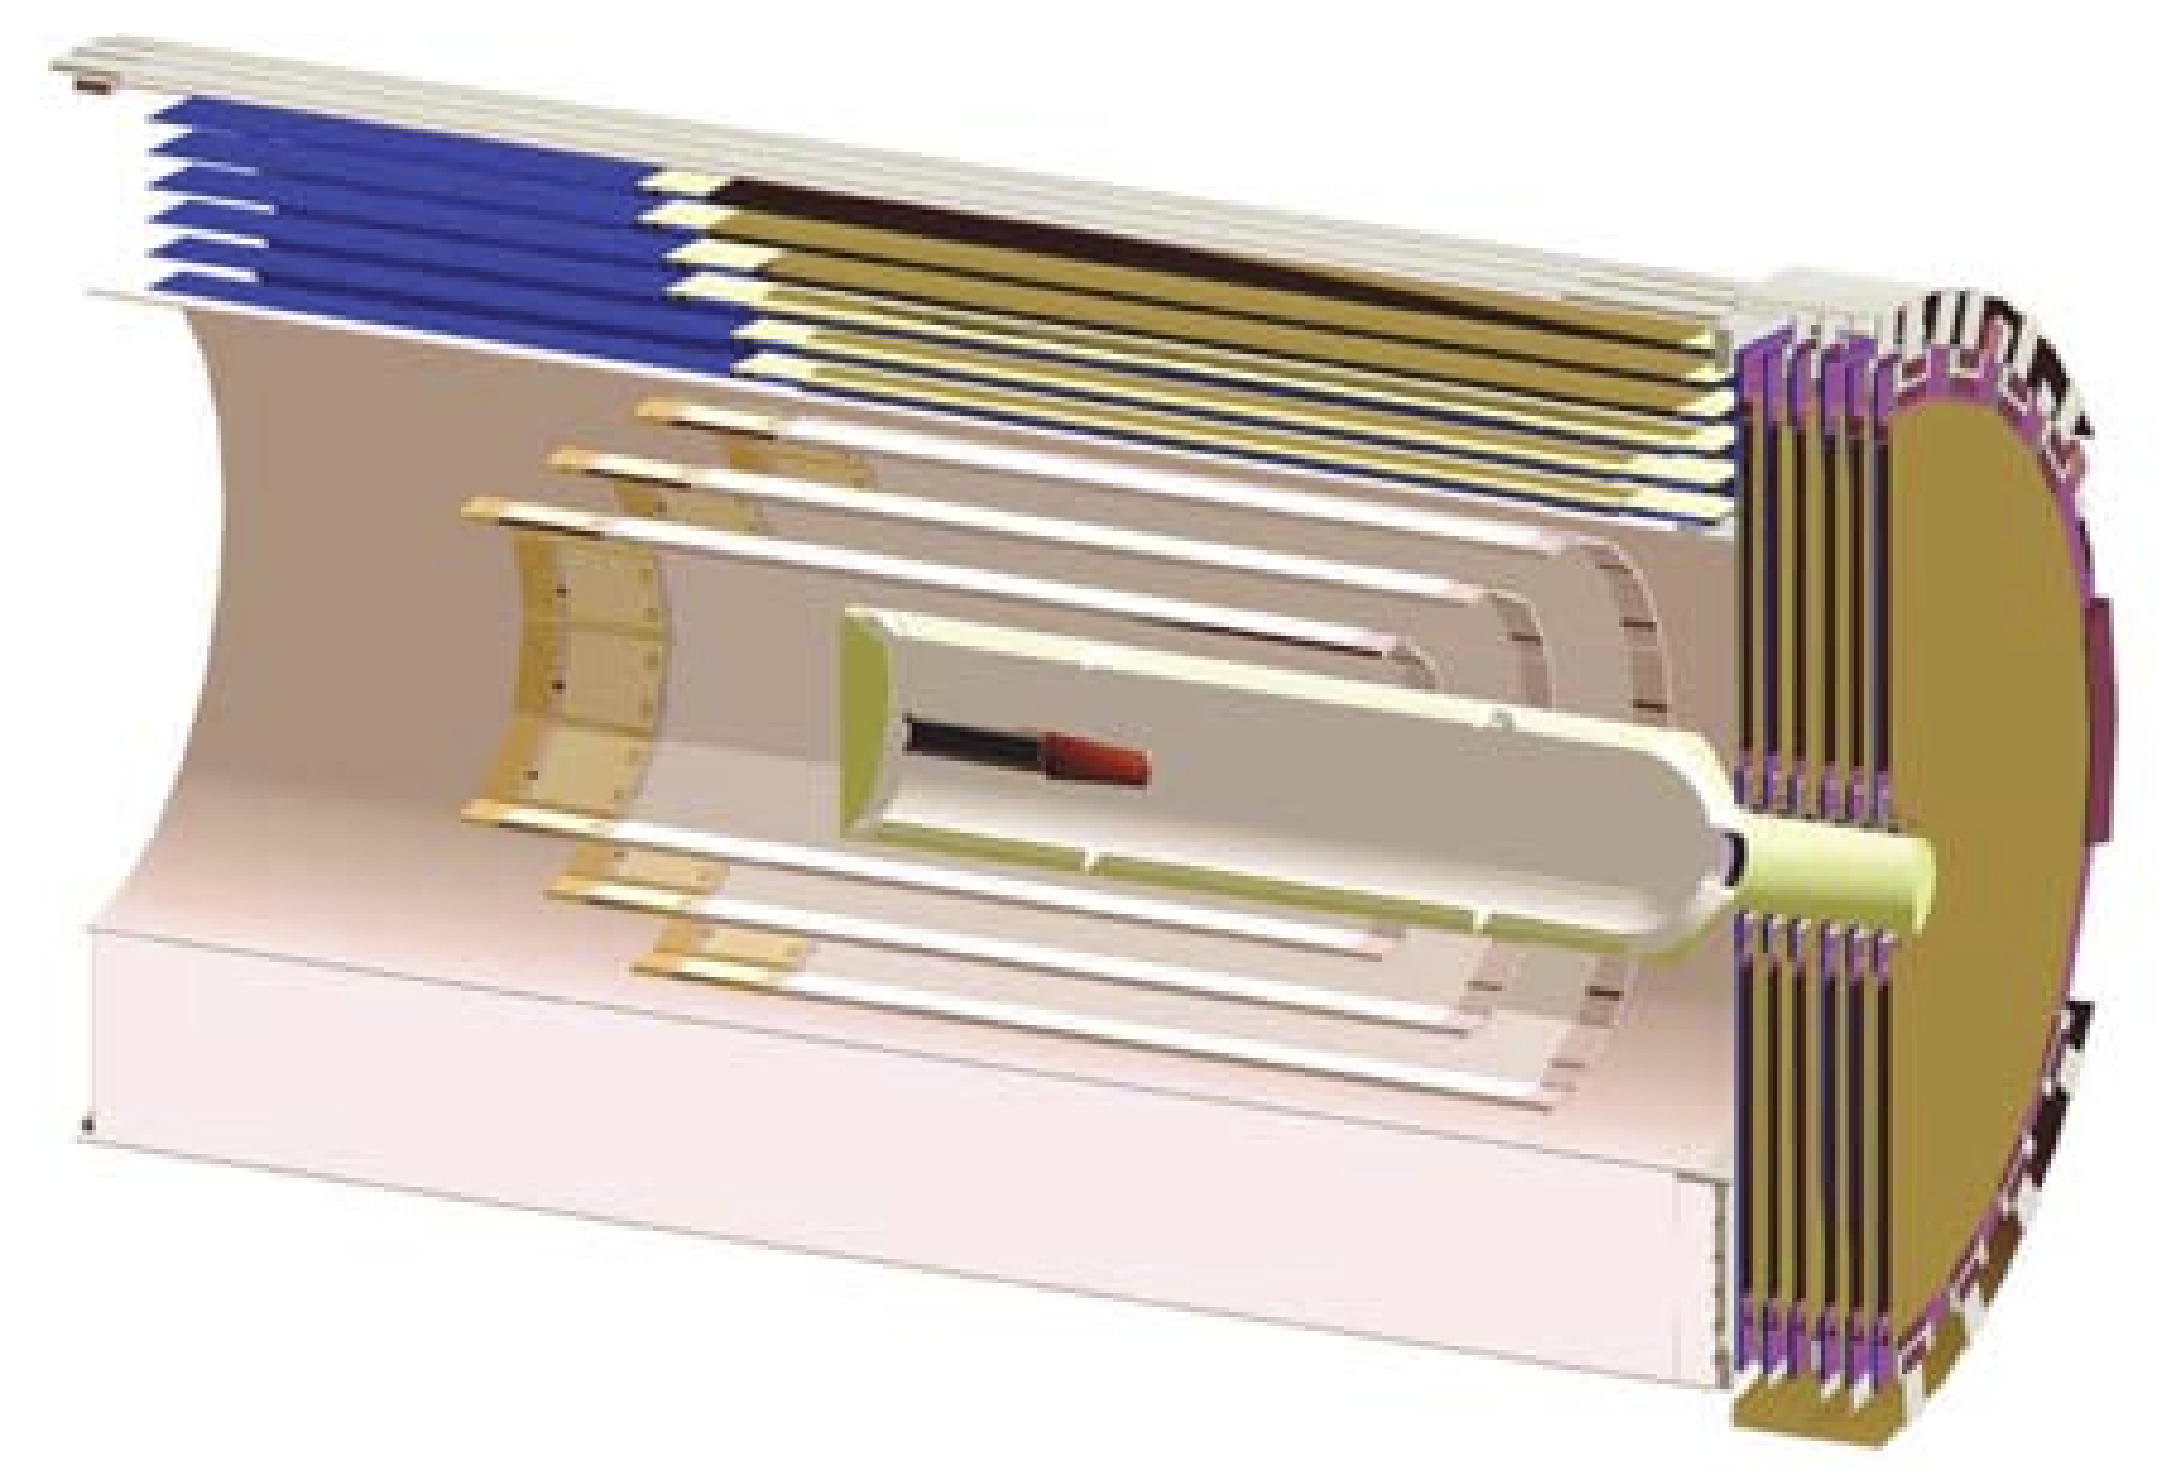
\includegraphics[width=0.3\textwidth]{Chapters/Ch2-Experiment/clas-12-exp/clas-detectors/cd/pics/CVT.png}\label{fig:mvt}
            }
            \hfill
            \subfloat[The CD, in retracted position for maintenance.]{
                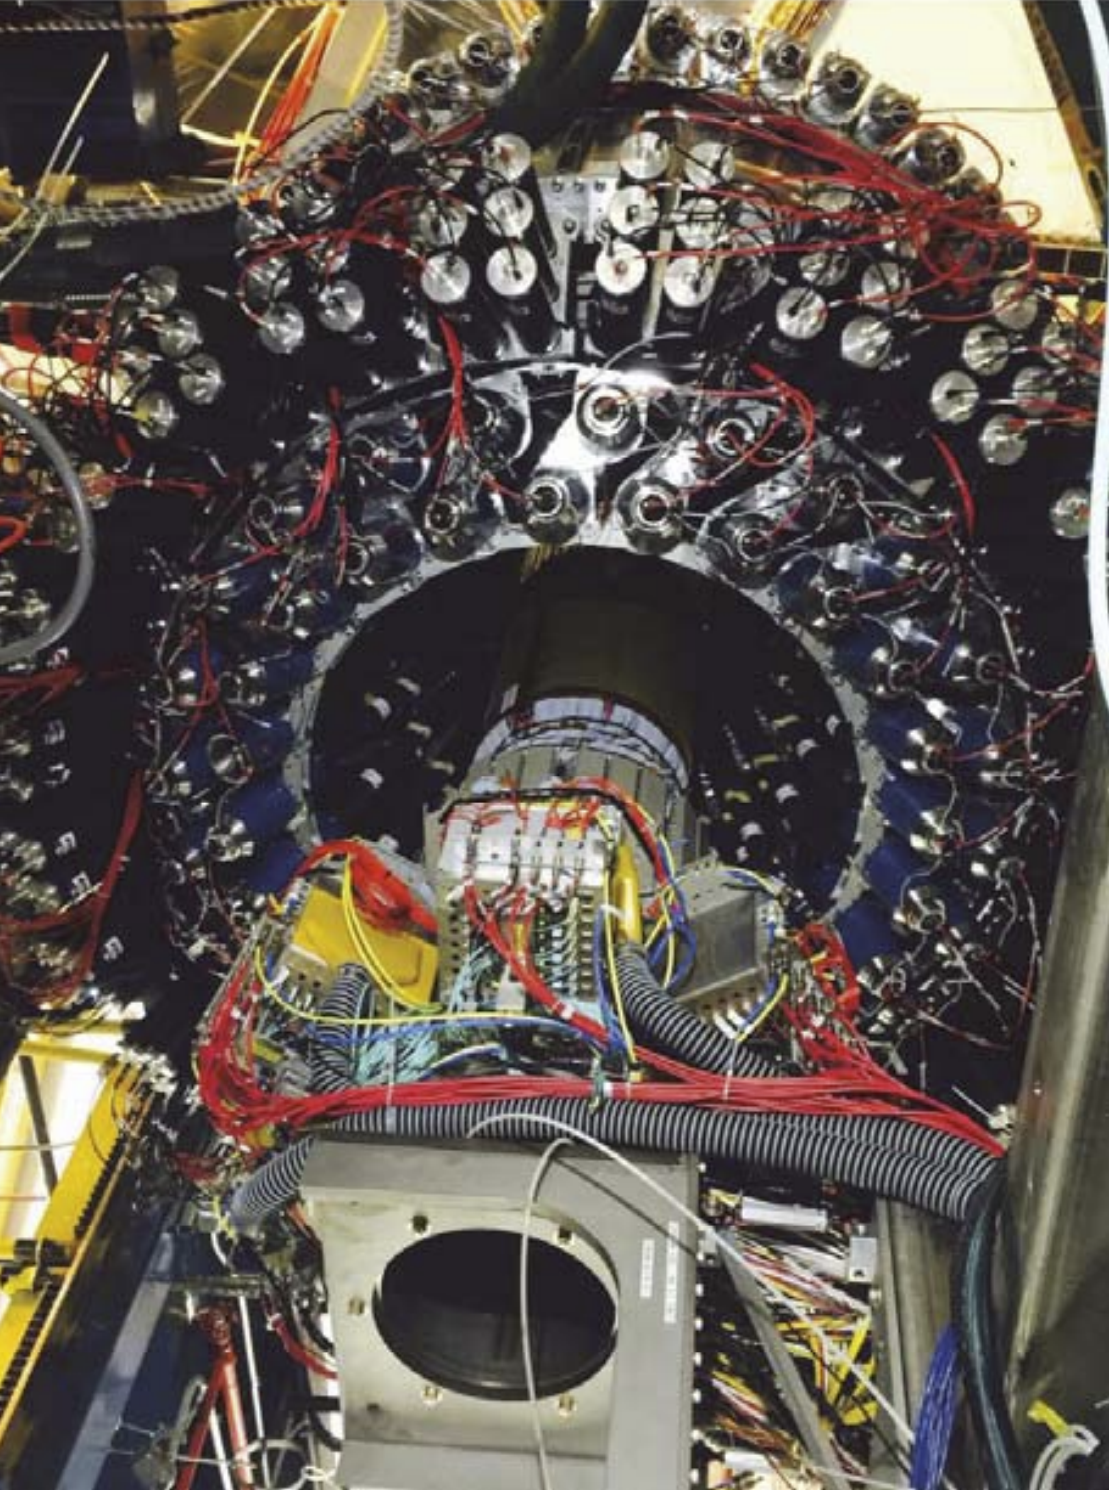
\includegraphics[trim={0 5cm 0 0},clip,width=0.3\textwidth]{Chapters/Ch2-Experiment/clas-12-exp/clas-detectors/cd/pics/real_CD.png}
            }
            \caption[Central Detector Packages]{Models of the CTOF (a) and CVT (b) and their physical realizations in the CD (c). Note the first three inner cylindrical layers of the CVT (b) correspond to the SVT, the outer six to the BMT, and the right end cap six to the FMT. Images from \parencite{Burkert2020TheLaboratory}.}
            \label{fig:your_labels}
        \end{figure}
     
        

\subsubsection*{Other System Components}

    At very low beam angles ($2.5^{\circ}$-$4.5^{\circ}$) there is the Forward Tagger (FT) \parencite{Acker2020TheTagger} which contains a tracker, homogeneous calorimeter, and hodoscope. At the other end of the beamline ($155^{\circ}$-$175^{\circ}$) there is the Backward Angle Neutron Detector (BAND)  \parencite{Segarra2020TheBAND}, which is not relevant for this analysis. Furthermore, the BAND and the Forward Micromegas Tracker (FMT)  \parencite{Acker2020TheTracker} were not installed at the time the data for this analysis was taken, although they have since been commissioned. 
    
    

\iffalse
%To possibly encorporate

    \begin{figure}[H]
        \centering
        \subfloat[]{
            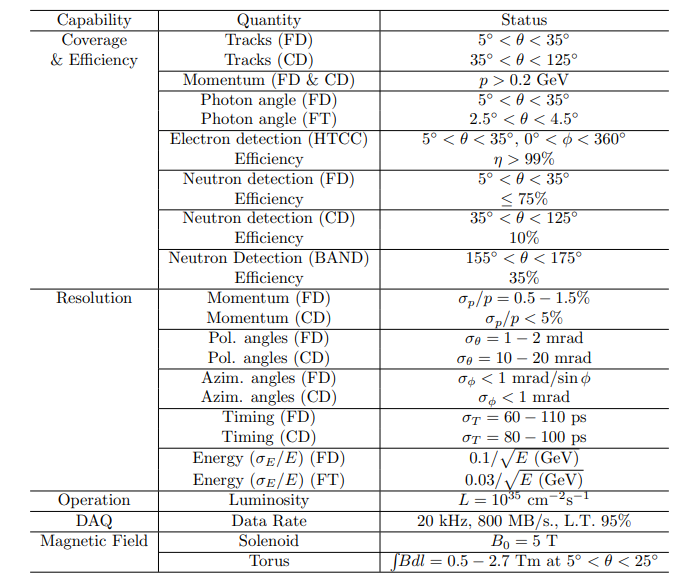
\includegraphics[width=0.3\textwidth]{Chapters/Ch2-Experiment/clas-12-exp/clas-detectors/other/pics/clas12-params.png}
        }
        \hfill
        \subfloat[]{
            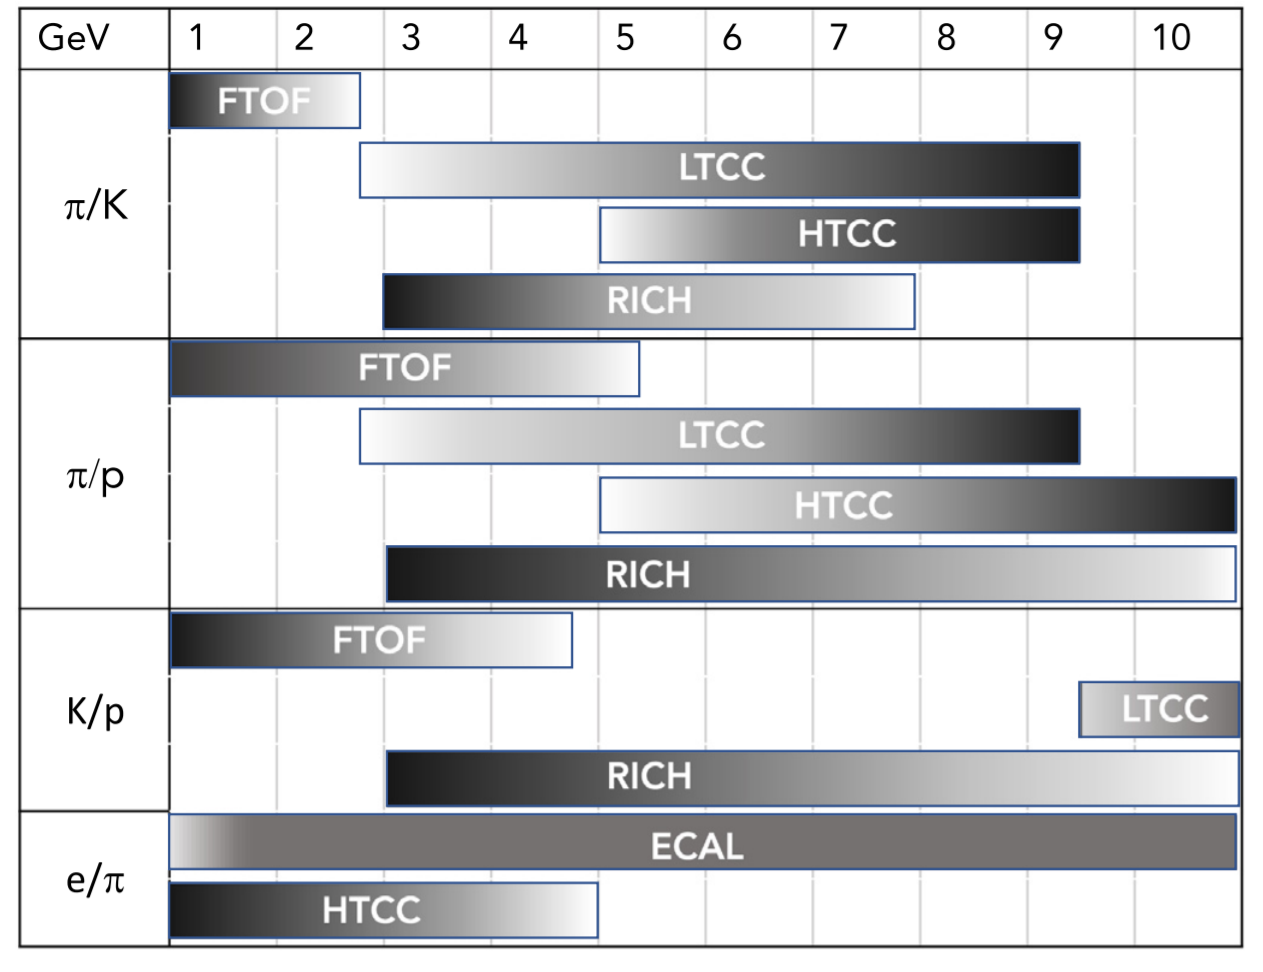
\includegraphics[width=0.3\textwidth]{Chapters/Ch2-Experiment/clas-12-exp/clas-detectors/other/pics/pid-clas12.png}
        }
        \hfill
        \subfloat[]{
            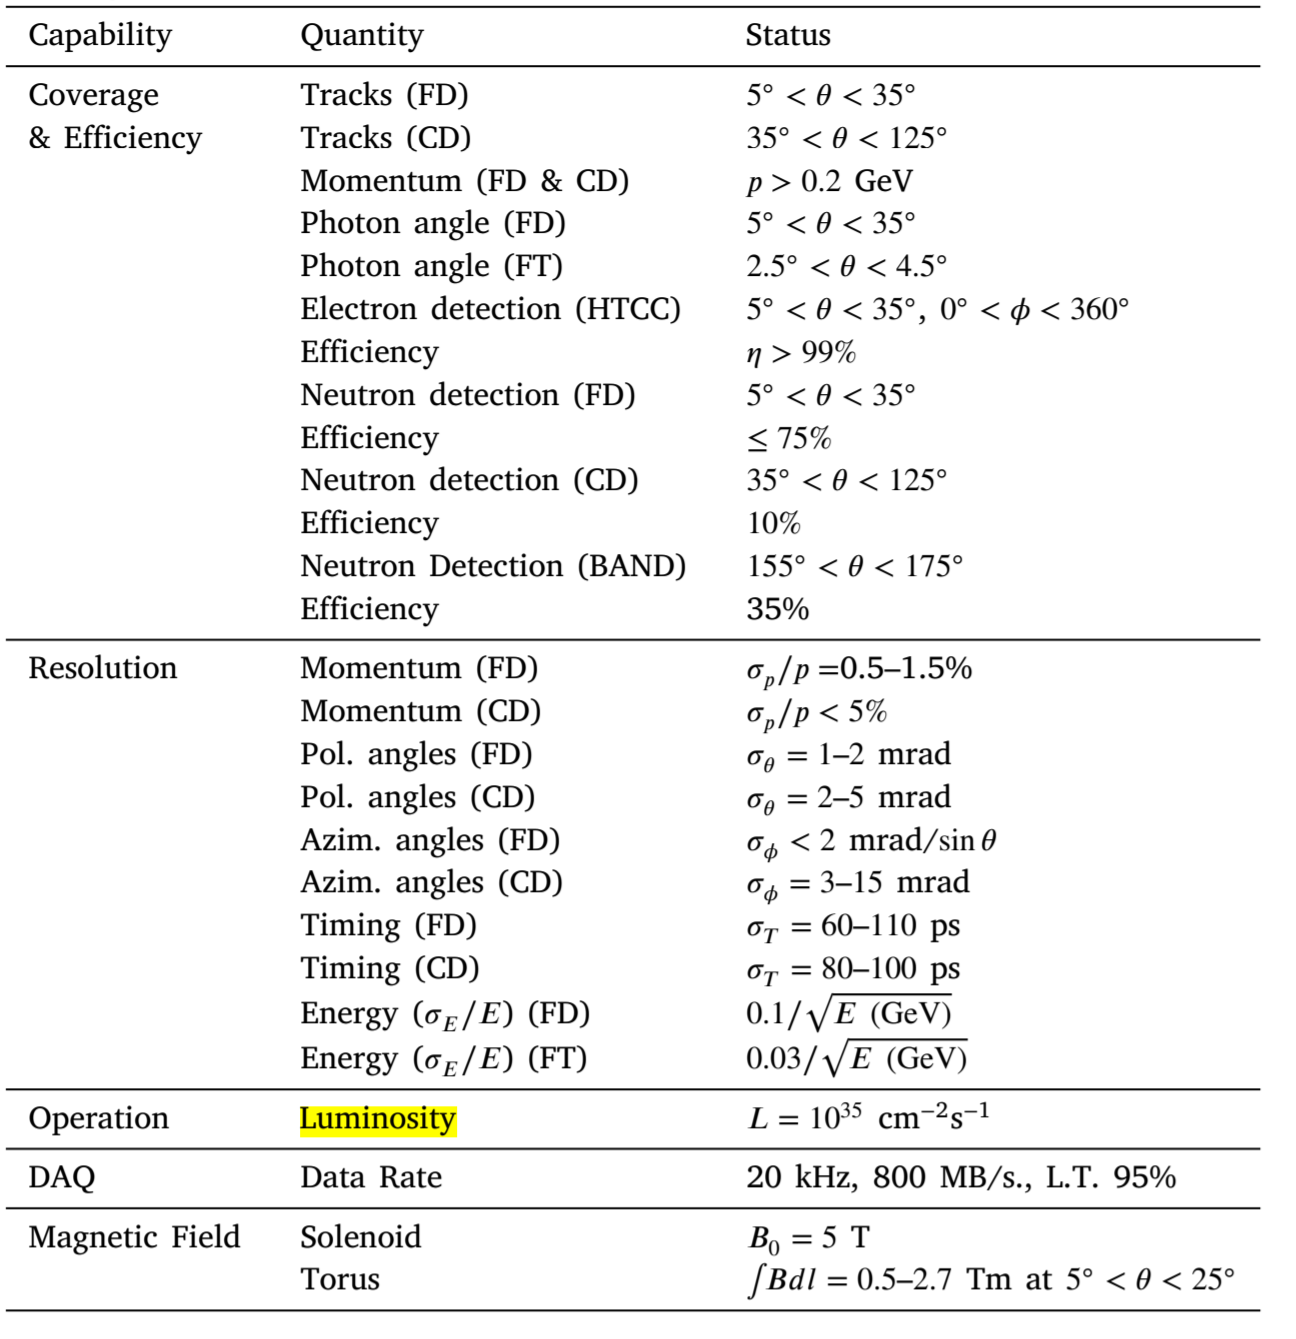
\includegraphics[width=0.3\textwidth]{Chapters/Ch2-Experiment/clas-12-exp/clas-detectors/other/pics/specs-v2-clas12.png}
        }
        \caption{Your caption goes here}
        \label{fig:others}
    \end{figure}

    
    %From sangbaek
    The Data Acquisition (DAQ) \parencite{Boyarinov2020TheSystem} dead-time can be corrected by using a gate at the FC that closes when the DAQ procedure is complete \parencite{Baltzell2020ThePerformance}. The total charge regardless of the gate is called the ungated charge, and the charge collected during the gate on is the gated charge. The ratio of the gated charge to the ungated charge is recorded as the DAQ live-time. The complete listing of detector components can be found in Table. 2.1. The CLAS12 detector components relevant to the particle 4-momentum vector reconstruction are grouped by their characteristics in Table. 2.2. The essential properties like threshold and resolutions and the prominent material components are also listed. 



    Table 2.2: The properties of the relevant subdetectors for the DVCS analysis. The
    properties relate mostly to the effective measurement uncertainties listed in each NIM
    article [135, 136, 140, 141, 143, 144, 147, 152].
    
    \begin{table}[ht]
        \centering
        \begin{tabularx}{\textwidth}{XccXX}
        \toprule
        Name & Coverage ($^\circ$) & Nominal Property & Material \\
        \midrule
        HTCC & 5-35 & $0.015 < p < 4.9$ GeV/c & CO$_2$ \\
        FTOF 1B & 5-35 & $60 - 110$ ps (t) & \\
        FTOF 1A & 5-35 & $90 - 180$ ps (t) & Plastic \\
        FTOF 2 & 35-45 & $170 - 180$ ps (t) & Scintillator \\
        CTOF & 35-125 & $80$ ps (t) & \\
        ECAL & 5-35 & $10\%/\sqrt{E}$ (E) & Pb (absorber) \\
        & & $1.2$ mrad ($\theta, \phi$) & Plastic scintillator \\
        FT-Cal & 2.5-4.5 & $2\%/\sqrt{E} \oplus 1\%$ (E) & PbWO$_4$ crystal \\
        & & $1.5\%$ ($\theta$) & \\
        & & $2^\circ$ ($\phi$) & \\
        DC & 5-40 & $1\%$ (p) & Aluminium wire \\
        & & $1$ mrad ($\theta$) & $90\%$ Ar \\
        & & $1$ mrad/sin $\theta$ ($\phi$) & $10\%$ CO$_2$ \\
        CVT & 35-125 & $5\%$ ($p_t$) & SVT: Si \\
        & & $10 - 20$ mrad ($\theta$) & BMT: $90\%$Ar + $10\%$C$_4$H$_{10}$ \\
        & & $5$ mrad ($\phi$) & \\
        FC & - & $0.48\%$ (L) & Pb \\
        \bottomrule
        \end{tabularx}
        \caption{Caption}
        \label{tab:my_label}
    \end{table}


\fi


    
\subsection{Experiment Run Conditions}
    
The 499 MHz beam structure equates to a signal with a period of 2.004 ns. In practice, the beam was delivered in every other RF bucket, and so bunched at a period of 4.008 ns.

       
            CLAS12 runs with "open trigger", which means different sub-experiments can define their own triggering logic. There is a standard electron trigger, based off of hits in HTCC, ECal, and FTOF. 

        Only about 50\% of the electron triggers recorded with an inbending torus polarity are actually electrons. For outbending torus polarity, hte electron trigger purity is as high at 70\%. 
    
    \href{https://www.jlab.org/Hall-B/clas12-web/}{Detector Specs}
    
    20 kHz Level 1 trigger rate, 1 GB/s.

   The CLAS12 detector is a large angle spectrometer that generally covers angles from 5 to 130 degrees, spanned by two main detector subsystems - the Forward Detector and the Central Detector.

    
   CLAS12 at the design luminosity of 1035 cm−2 s−1

        Data taken is RGA taken in Fall 2018

        Mention configurations and combinatorics


%from sangbaek
In fall 2018, two sets of experiments have been performed with opposite toroidal magnetic field directions
keeping the other detector settings the same. The toroidal magnet bends the scattered
trigger electron inward or outward along the beam direction. In convention, the torus
polarity associated with the inwardly bending electrons is called the negative, -1,
-100\%, or inbending polarity. The opposite is called the positive, +1, +100\%, or
outbending polarity. Both experiments took data with the beam energy of 10.6 GeV,
and the beam current of about 50 nA. The effects due to the variation in the beam
current during the run periods will be taken into account at the end of the analysis.
The CLAS collaboration performed other CLAS12 experiments with different targets
like liquid deuterium, and various beam energies. The description in this thesis
will be focused on the RG-A fall 2018.

The measured
electron beam polarization was 86.9\% during the RG-A data taking in fall 2018.



\section{Reconstruction and Particle Identification}
    here we talk about CLAS PID
\subsection{Decoding and Track Reconstruction}\label{sec:decrec}

\subsection{Particle Identification}


For this analysis all final state particles should be detected.
After $\pi^0$ decay we are going to have 4 particles: electron, proton and two photons.
The particle identification methods are applied to select the exclusive event with at least one electron, proton and two photons. 


    \subsubsection{Electron}
    \subsubsection{Proton}
    \subsubsection{Photon}
    \subsubsection{Pion}
    
    Basic event builder cuts are utilized, then additional cuts are made that are common with the RGA Analysis note (\href{https://www.overleaf.com/project/5ea737720942930001ff5e9c}{overleaf link} and developed by Sangbaek Lee (sangbaek@mit.edu - \href{https://github.com/Sangbaek/analysis_code/tree/analysis/pid}{github code here}. For this analysis, both the central detector and forward detector are utilized for proton tracking. The forward tagger is also utilized for photon identification. 
    


\subsubsection{Neutral pion}
    In addition to individual particle PID procedures the cut on the mass of two photons is applied:
    \begin{itemize}
    	\item $0.07<M_{\gamma\gamma}<0.2$ GeV
    \end{itemize}
    The pion is more thoroughly constrained by the exclusivity cuts, described in the next section.
    

\begin{figure}[hbt]
	\centering
	\includegraphics[page=6,width=0.6\textwidth]{Chapters/Ch4-BaseAnalysis/pid_figs/eppi0.exclusive.pdf}
	
	\caption{The distribution for mass of two photons $M_{\gamma\gamma}$}.
	\label{fig:ggmass}
	
	\centering
	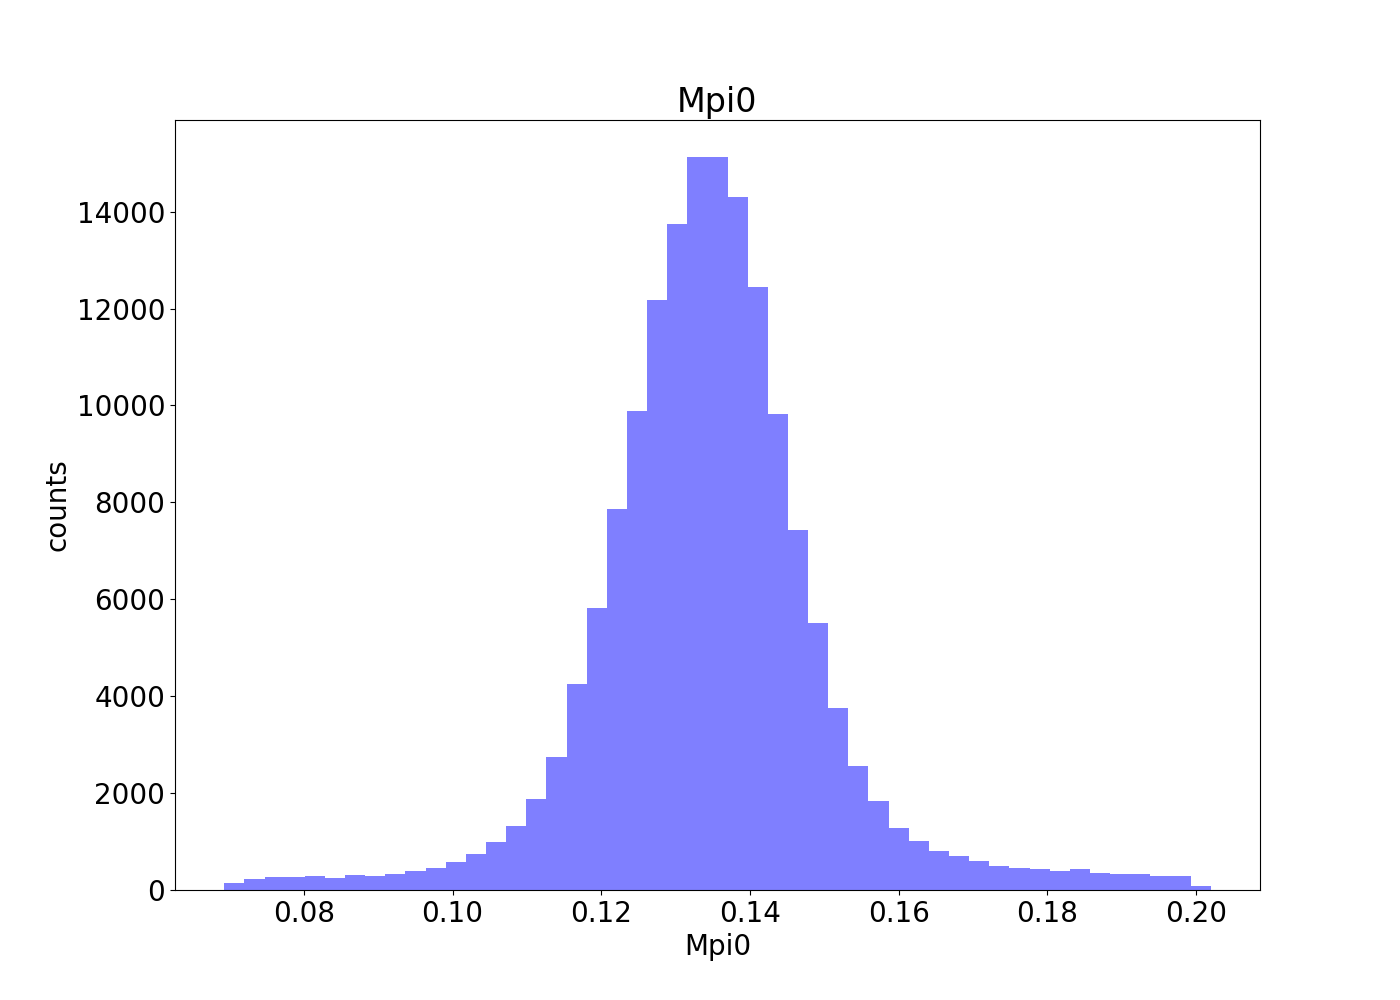
\includegraphics[width=0.6\textwidth]{Chapters/Ch2-Experiment/recon_pid/pid_figs/Mpi0.png}
	
	\caption{The distribution for mass of two photons after exclusivity cuts}.
	\label{fig:ggmass_after}
	
\end{figure}




\subsection{Data Storage and Formatting}
    \subsubsection{Data Location and Availability}
    \subsubsection{File Formatting and Conversion}\label{sec:filtering}
        Mention that same transformations are used for rec events and filtering
    

    






